\section{gitc extension}
\label{sec:Extension}
In this section we describe how a cloud9 user can work with our extension and we show how the developing workflow is improved by it.
Further we compare our extension to other tools introduced in section~\needcite{related work}.
Finally we will explain how we intregrated our extension to cloud9 and how we implemented it.

\subsection{Description}
\paragraph{The editor adjustments} of our extension will promt the cloud9 user immediately with visiual feedback of source code changes.
That means while typing within the editor annotations will appear next to the left grutter line as can be seen in figure~\ref{fig:editor}.

The changes show the staged and unstaged changes of the git repository respectively.
We choose to display those both types of changes as colored annotations whereas the already staged changes are more transparent.
In the upper screenshot of the cloud9 editor are only unstaged changes displayed.
The lower screenshot shows that the state of the git repository is changed.
Some of the changes are staged and at~\circnum{2} and~\circnum{3} are some (new) unstaged changes.
So in the line marked by~\circnum{2} there are both staged and unstaged changes visualized.
The colors green, blue and red are used to visualize added~\circnum{3}, changed~\circnum{2} and deleted~\circnum{1} lines respectively.

Furthermore the user will get tooltips hovering over one annotation.
In this way deleted lines or the old content of changed lines will be displayed to the user.
We do not provide buttons to stage, unstage or discard the changes because there is already an extension which allows developers to go back in history (see figure~\ref{fig:history}).
As for the staging and unstaging we want to have an overview over all current changes and thus rather use the diff view than search in single source code files for changes.

\begin{figure}
   \centering
   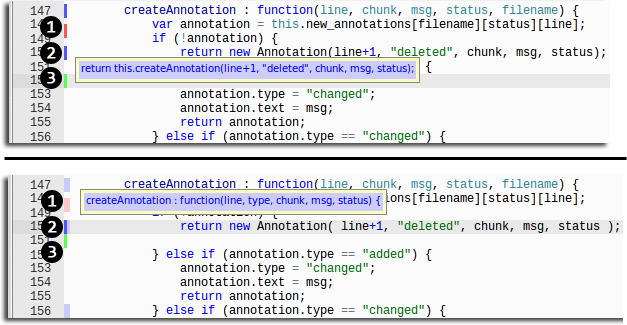
\includegraphics[width=0.9\textwidth]{images/extension_tooltip_comparison.png}
   \caption{Editor adjustments of our cloud9 extension gitc.}
   \label{fig:editor}
\end{figure}

\paragraph{Using our diff view} the cloud9 developer has now a view to explore \texttt{git diff} visually.
By clicking on the pane button \circnum{1} in figure~\needcite or simply using the keyboard shortcut \texttt{strg + g} or \texttt{cmd + g} ....

\begin{figure}
   \centering
   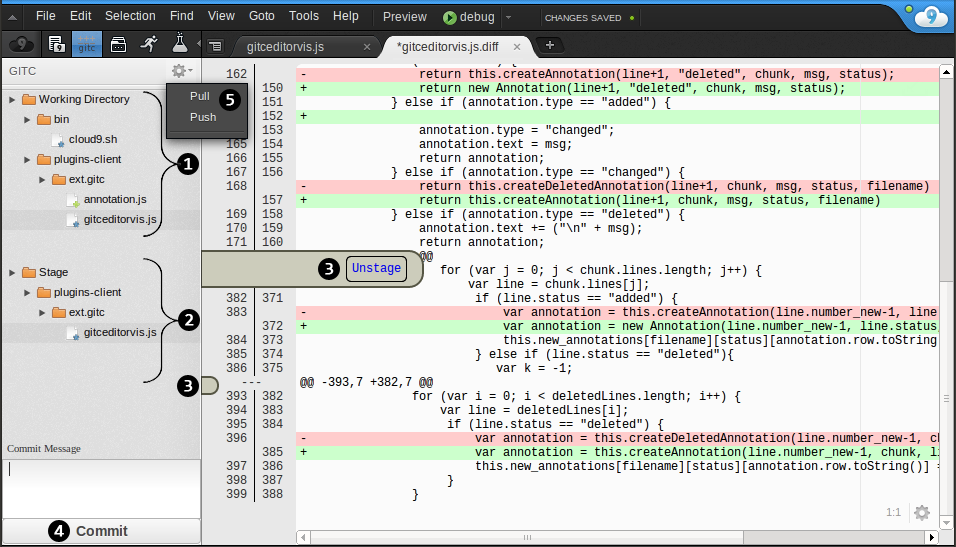
\includegraphics[width=0.9\textwidth]{images/extension_unstage.png}
   \caption{The diff view of our cloud9 extension gitc.}
   \label{fig:diff_view}
\end{figure}

comparison to earlier editing way, mention history extension (and why we have choosen not to implement stage etc buttons here)
comparison to earlier diffing, committing

comparison to related work

\subsection{Implementation}
In the following subsections we will describe how we implemented our extension.
First we will have a closer look at how we intregrated our extension to cloud9 and how we execute git commands.
Then we will explain how we implemented the adjustments in the cloud9 editor and the new diff view.

\subsubsection{Integration to cloud9}
%Stephi

\subsubsection{Editor Adjustments}
%Patrick

\subsubsection{Diff View}
%Markus
